\newpage
%\null
%\cleardoublepage



%************************************************************************************************
% Kap.4 Programmentwicklung
%************************************************************************************************

\chapter{Programmentwicklung}
\label{chap:Programmentwicklung}
Bei der Programmentwicklung werden die in Kap. \ref{chap:modellbildung} aufgestellten Gleichungen mit Matlab und Simulink umgesetzt.
Es wird begonnen, die Gleichungen des elektrischen und des mechanischen Teils des Motors in Simulink umzusetzen.
Im Anschluss folgt die Implementierung der Werte, des Simulinkprogrammes und des Motors in Matlab.
Daran schliesst sich die Umsetzung der Sensoren in Matlab.
Wenn die Sensoren mit Matlabfiles eingebunden werden k�nnen, werden die Simulink- und Matlabprogramme des Motors entsprechend erweitert.

\section{Motor in Simulink}
\label{chap:motorinsimulink}
Es werden die Formeln \ref{equ:motorspannungsimulink} und \ref{equ:motormomentsimulink} aus den Kap. \ref{chap:elekteil} und \ref{chap:mechteil} hergenommen.
Durch ein umstellen der beiden Formeln, so dass nur noch erste Ableitungen in beiden Formeln vorkommen, lasen sie sich kombinieren und in Simulink einbinden, da so ein
Gleichungssytem nur mit ersten Ableitungen entstanden ist.
Um einen besseren �berblick zu bekommen, werden die Formeln hier noch einmal aufgef�hrt.
\begin{center}
\begin{equation}
\label{equ:motorspannungsimulink2}
si_A = \frac{1}{L_A} (e_A - R_Ai_A + u_e)
\end{equation}
\end{center}
\begin{center}
\begin{equation}
\label{equ:motorspannungsimulinkkonst2}
e_a = K_M * \Phi \omega
\end{equation}
\end{center}
\begin{center}
\begin{equation}
\label{equ:motormomentsimulink2}
s\omega = \frac{1}{J} (M_M - r * \omega - M_L)
\end{equation}
\end{center}
\begin{center}
\begin{equation}
\label{equ:motormomentsimulinkkonst2}
M_M = K_M * \Phi *i_A
\end{equation}
\end{center}
$K_M$ und $\Phi$ sind Motorkonstanten.

Mit der Annahme das 
\begin{center}
\begin{equation}
\label{equ:variablensimulink1}
x_1 := \omega
\end{equation}
\begin{equation}
\label{equ:variablensimulink2}
x_2 := i_A
\end{equation}
\end{center}
ist, l�sst sich folgendes Gleichungssytem aufstellen:
\begin{center}
\begin{equation}
\label{equ:motormomentsimulink1}
\dot{x_1} = \frac{1}{J} (K_M \Phi x_Sensor_Funktion2 - r * x_1 - M_L)
\end{equation}
\begin{equation}
\label{equ:motormomentsimulink1}
\dot{x_2} = \frac{1}{L_A} (K_M * \Phi x_1 - R_Ax_2 + u_e)
\end{equation}
\end{center}
Dieses Gleichungssytem l�sst sich jetzt durch die grafischen Elemente in Simulink sehr einfach modellieren.

Wie zu Begin des Kap. \ref{chap:motor} erw�hnt, war es nicht m�glich an verschiedene Werte der Motorkonstanten $K_M$ und $\phi$ zu gelangen.
Aus diesem Grund wird auf die begleitenden Unterlagen der Vorlesung Systemtechniken von Prof. Froriep zur�ck gegriffen.

Auf dieser Grundlage werden die weiteren Programme entwickelt.

Um eine Regelung aufzubauen, wird noch ein Regler, ein Sollwertgeber und ein Subtrahierer von Ist- und Sollwert ben�tigt.
Diese werden �ber die Simulinkbibliothek eingebunden und entsprechende Verbindungen werden angelegt.
Das fertige Grundprogramm ist in Abb. \ref{fig:grundprogramm} dargestellt.
\begin{figure}[!h]
	\centering
	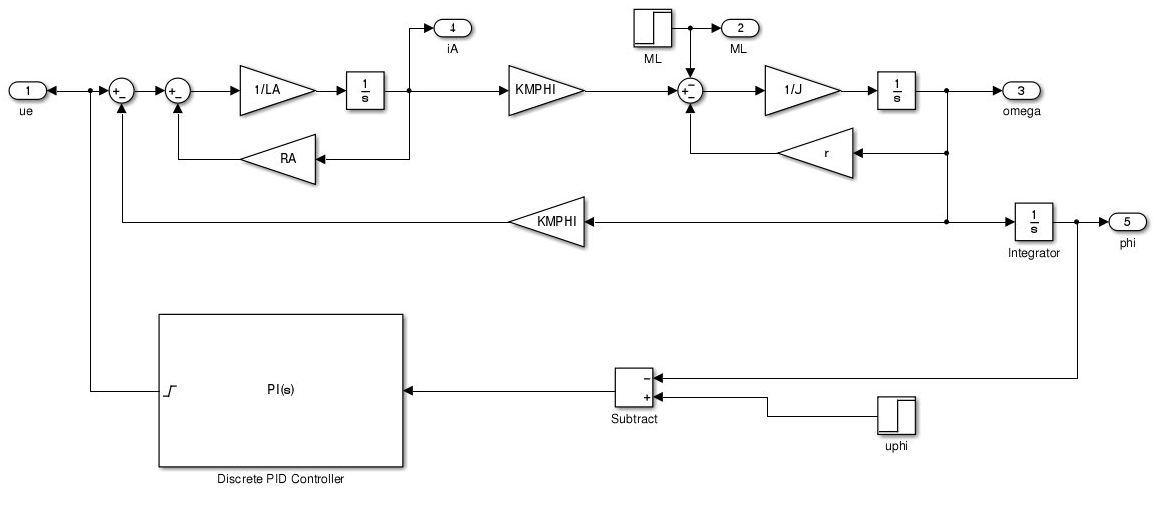
\includegraphics[width=0.6\textwidth]{sSpiegel.jpg}
	\caption{Simulink Grundprogramm}
	\label{fig:grundprogramm}
\end{figure}

\section{Matlab}
\subsection{Motor in Matlab}
Die Programmentwicklung in Matlab gestaltet sich f�r den Motor als relativ einfach, da, wie oben erw�hnt, keien Motordaten gefunden wurden, wird auf das Matlabfile von Prof. Froriep aus der Vorlesung "Systemtechniken" zur�ck gegriffen.
In diesem Matlabfile stehen:
\begin{itemize}
\item Die Motorkenndaten
\item Die berechnete Tr�gheit des Spiegels
\item Das berechnete Drehmoment
\item Die Grenzen f�r die Plots
\item Die Anweisungen f�r die Plots
\item Die Anweisungen f�r den Integrationsalgorithmus.
\end{itemize}

Dieses File ist eine sehr gute Grundlage f�r die Simuation, welches w�hrend der Simulation entsprechend angepasst werden kann.

Als Gr��en zur Ausgabe in einem Diagramm, interessieren vor allem die Eingangsspannung $u_e$, der aktuelle Winkel $\phi$, sowie der Sollwinkel mit seinen Toleranzen.
Es werden drei Plots dargestellt.
In dem ersten Plot ist die Motorspannung dargestellt.
In dem zweiten Plot der aktuelle Winkel $\phi$, der direkt von dem Motor abgegriffen wird, sowie der einzustellende Sollwinkel dargestellt.
Der dritte Plot enth�lt auch wieder den aktuellen Winkel $\phi$, jedoch mit einer feineren Aufl�sung um den Sollwinkel, um die Toleranzgrenzen besser erkennen zu k�nnen.

\subsection{Sensor in Matlab}
Der Sensor selbst wird nur mit Matlabprogrammen simuliert.
Dies erm�glicht verschiedene Sensoren in das Hauptprogramm einzubinden und �nderungen an z.B. den Ausma�en und dem Verhalten des Sensors vorzunehmen, ohne das Hauptprogramm �ndern zu m�ssen.

\subsubsection{Vorbereitungen}
Um einen Sensor mit seinen verschiedenen Kenngr��en wie Sensorfl�che, �bertragungsverhalten, und weiteres simulieren zu k�nnen, werden die verschiedenen Funktionen aus
Kap. \ref{chap:sensor}in einzelnen Matlabfiles gespeichert. 
Dieses macht die Aufgabenl�sung zwar komplexer, bietet aber den Vorteil, einzelne Bereiche f�r sich testen zu k�nnen, bevor sie in den Sensor eingebunden werden.

\subsubsection{Files}
Ich w�rde hier evtl. schreiben, in welche Unterprogramme Du den Sensor aufgeteilt hast.
Auch sollten Deine Versuchsprogramme erw�hnt und mit in den Anhang kommen.
Da steckt viel Arbeit drin und war/ist f�r die Simuation �u�erst wichtig.